\uuid{A03B}
\exo7id{7128}
\auteur{megy}
\organisation{exo7}
\datecreate{2017-02-08}
\isIndication{false}
\isCorrection{true}
\chapitre{Géométrie affine euclidienne}
\sousChapitre{Géométrie affine euclidienne du plan}

\contenu{
\texte{
% tags : chasse aux angles, un peu plus difficile

Soit $\mathcal C$ un cercle, $[BC]$ une corde, et $A \in \mathcal C$ tels que les arcs $AB$ et $AC$ soient égaux. Soient $[AD]$ et $[AE]$ deux autres cordes d'extrémités $A$, qui coupent $[BC]$ en $F$ et en $G$, respectivement. Montrer que $DEFG$ est inscriptible.
}
\reponse{
Traçons une figure :

\begin{center}
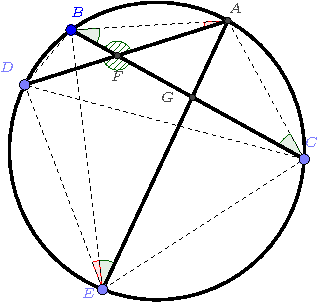
\includegraphics{../images/img007128-1}
\end{center}


\emph{[Sur la figure, on voit que les angles $\widehat{GFD}$ et $\widehat{GED}$ sont supplémentaires, car $\widehat{GFD}=\widehat{BFA}$ et $\widehat{GED}=\widehat{GEB}+\widehat{BED} = \widehat{FBA}+\widehat{BAF}$. Il ne reste plus qu'à rédiger cette preuve un peu plus rigoureusement avec des angles de droites.]}

Montrons que $(FD,FG)=(ED,EG)$, ce qui prouve que $EDFG$ est inscriptible.

Tout d'abord, comme $(FD)=(FA)$ et $(FG)=(FB)$, on a 
\[(FD,FG)=(FA,FB).\]

Ensuite, la somme des angles du triangle $ABF$ vaut $\pi$, donc en termes d'angles de droites on a la relation 
$(FA,FB)+(AB,AF)+(BF,BA)=0$, c'est-à-dire:
\[
(FA,FB) = (AF,AB)+(BA,BF).
\]
Calculons chacun de ces deux angles. D'une part, on a :
\begin{align*}
(AF,AB) &= (AD,AB) \text{ car $(AD)=(AF)$}\\
&=(ED,EB) \text{ car $ABDE$ est inscriptible}.
\end{align*}
Et d'autre part :
\begin{align*}
(BA,BF) &= (BA,BC) \text{ car $(BF)=(BC)$} \\
&= (CB,CA) \text{ car $ABC$ est isocèle en $A$}\\
&= (EB,EA) \text{ car $ABCE$ est inscriptible.}
\end{align*}

Finalement, on obtient donc:
\begin{align*}
(FD,FG)&=(FA,FB) \\
&= (AF,AB)+(BA,BF) \\
&= (ED,EB) + (EB,EA)\\
&= (ED,EA)\\
&= (ED,EG) \text{ car $(EG)=(EA)$,}
\end{align*}
ce qu'il fallait démontrer.
\begin{center}
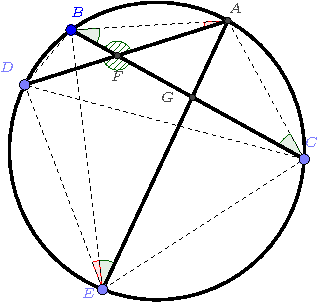
\includegraphics{../images/img007128-1}
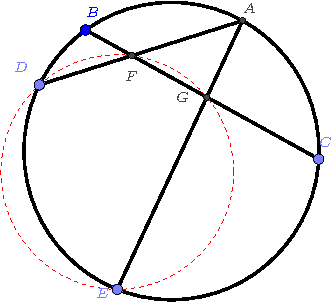
\includegraphics{../images/img007128-2}
\end{center}
}
}
